\section{Search}
The Zimbra Drive search feature appears upon selecting the drive item in the dropdown search menu or changing to the drive view.
The Zimbra Drive icon in the search toolbar means that the following search will be performed to the user own drive.
\begin{figure}[htbp,!h] 
\centering 
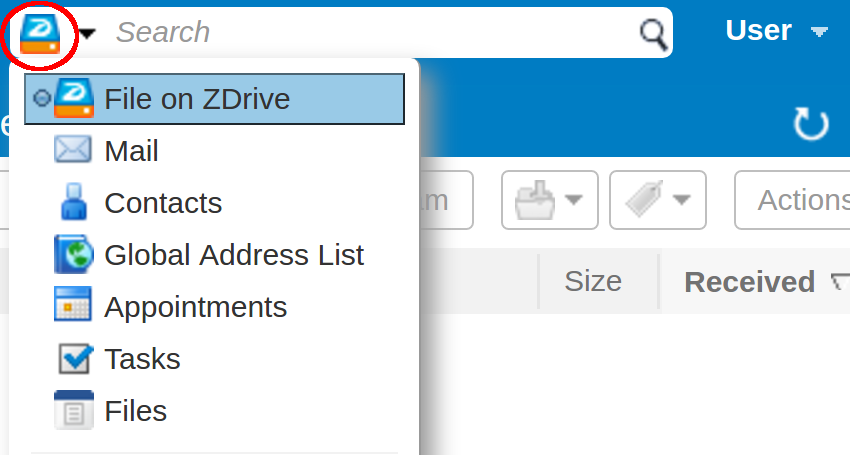
\includegraphics[scale=0.25]{\srcPath/images/ZD-searchMenu.png} 
\caption{Search Menu Item} 
\label{fig:searchMenu}
\end{figure}

The search feature has a location command and a string filter.\\
The location command is in the following:
\begin{verbatim}
in:"/Documents"
\end{verbatim}

\subsection{Search Folder Content}
